\chapter{Project Management}

\section{Process Model}

\begin{figure}[H]
  \centering
    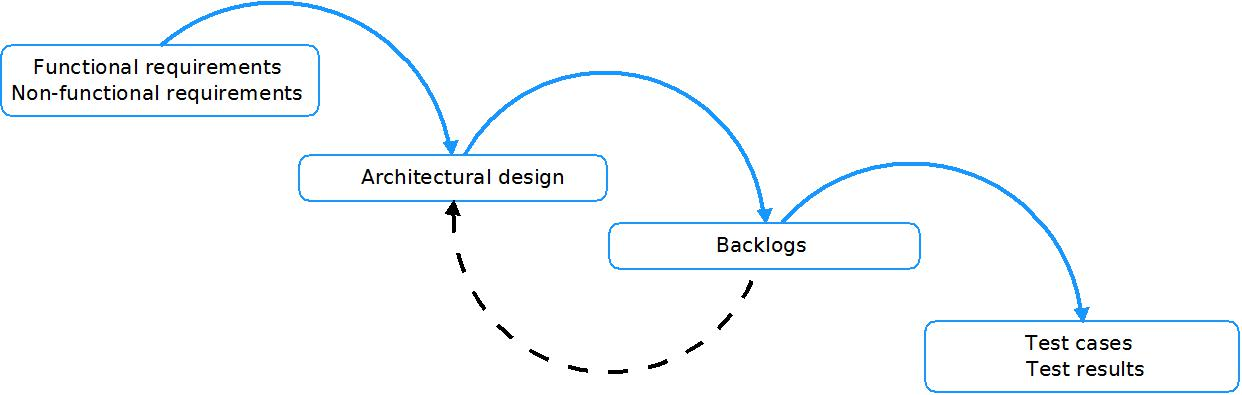
\includegraphics[width=1.0\textwidth]{img/waterfall.jpeg}
  \caption{Process model, 'Extended waterfall model'} 
  \label{fig:exwaterfall}
\end{figure}


Due to the extensive need for documentation, Scrum is not a suitable model of 
this process. Moreover, the intended model of process cannot be fitted in a 
waterfall model. Therefore, the model used will be a mixture of the best 
properties from both models. First of all the architecture will be designed 
along with the production of a detailed, sensible documentation. Then a simple, 
“bare bone” version of the game will be developed. Finally, the required 
features will be iterated on this version.


\subsection{Kanban board}

\begin{figure}[H]
  \centering
    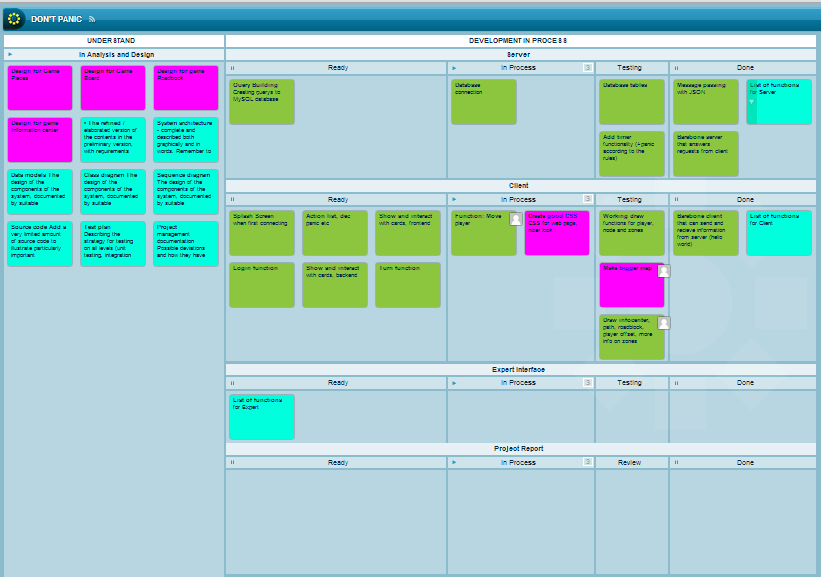
\includegraphics[width=1.0\textwidth]{img/kanban.png}
  \caption{Project management, 'KanBan board'} 
  \label{fig:kanban}
\end{figure}

The Kanban system fitted the project development process well, as a core 
prototype of the game was initially developed. Secondly, plans were made to 
add features such as a replay of a game session, an Expert interface and a 
database. It was decided to use an online version of a Kanban board called 
LeanKit Kanban. LeanKit was easy to use and enabled customizing the separation 
of tasks and processes on the board, as well as categorizing tasks by color. 
In addition, it enabled customizing the Kanban board, such as adding an extra 
“Testing” section for tasks.




\section{Roles and responsibilities}
These are the roles assigned to the different team members:

\begin{itemize} \setlength{\itemsep}{0cm}\setlength{\parskip}{0cm}
	\item Customer/supervisor contact - Sindre Svendsrud
	\item Server manager - Jim Frode Hoff
	\item LaTeX configuration manager - Jim Frode Hoff
	\item Client manager - Stian Aurheim and Jørgen Foss Eri
	\item Expert interface manager - Adrian Arne Skogvold
	\item Team manager - Jørgen Foss Eri
	\item Test manager- Jens Even Berg Blomsøy
	\item Database manager - Jens Even Berg Blomsøy
	\item Documentation manager - Sindre Svendsrud
\end{itemize}

The LaTeX configuration manager was handed to Jim because he was the only one with prior experience to LaTeX. The rest of the roles were handed to the person who wanted that specific role. This was done because none of the group members had any more experience or knowledge about the roles than any of the others.
\\\newline

\noindent\textbf{Customer/supervisor contact}\\ % \noident == quickfix
The customer/supervisor contact is responsible for the communication with the 
customer and the supervisor. It is important that he shares important 
information such as time and place for meetings with the rest of the group.
\\\newline
\textbf{Server manager}\\
The server manager is responsible for the development of the server. That does 
not mean he has to do all the coding himself, but he has to make sure that 
everything that needs to be done on the server side is done. The main task is 
to implement the game rules.
\\\newline
\textbf{LaTeX configuration manager}\\
The responsibility of the latex configuration manager is to export the project 
report to latex and configuration of github.
\\\newline
\textbf{Client manager}\\
The client manager is responsible for the development of the client. That means 
that he has to make sure that the client is displayed correctly. Typical work 
here is the drawing of objects such as draw player or draw node. 
\\\newline
\textbf{Expert interface manager}\\
The expert interface manager is responsible for the expert interface. The 
expert interface sets up the game. The main task is to implement a way for the 
expert to set up the game.
\\\newline
\textbf{Team manager}\\
The team manager is responsible for the progress of the project. He makes sure 
deadlines are met, meetings are attended and that the team members are engaged.
\\\newline
\textbf{Test manager}\\
The test manager is responsible for writing the tests of the system. He should 
also make sure that the tests are performed.
\\\newline
\textbf{Database manager}\\
The database manager is responsible for the database, that means the design of the database (ER diagram) and the implementation of the database. Typical work here is to make database queries. 
\\\newline
\textbf{Documentation manager}\\
The documentation manager is responsible for the documentation of the project. The main tasks are to create and maintain the structure of the report.




\section{Time plan}
A time schedule to view planned tasks and their deadlines has been created in a 
Gantt chart (available in Appendix ~\ref{appendix:A}). 
\\\newline
A short summary of the development can be seen as:\\
Version 1: Server game logic, client event handler, (simple) client view and 
communication module \\
Version 2: Addition of the administration interface and the expert client, 
extend view and game rule support\\
Version 3: Adaptation to other clients, extra features beyond the core \\

\subsection{Milestones} 
During the project there are certain milestones to be completed in time, both project report and technical milestones. \\
\newline
\textbf{Project report milestones}\\
10 February - Delivery - Project report: Preliminary version\\
15 March - Delivery - Project Report: Mid-semester version\\
19 April - Delivery - Project report: Final comments from supervisor\\
27 May - Delivery - Project report: Final version\\
\newline
\textbf{Technical milestones} \\
18 February - Barebone client that can communicate with the server \\
18 February - Barebone server that can communicate with the client\\
28 February - Basic prototype of the game\\
28 February - Database connection\\
11 March - Game v.1, a simple, working prototype of the game\\
22 March - Database queries\\
19 April - Expert interface for setting up the game\\
10 May - Game final\\
\newline
These are the code milestones which were set for the project in regards to the 
client/server/database functionality. The reason the milestones is in that 
order is because many of them depend on the milestones prior to them. \\


\section{Work breakdown structure}

\begin{figure}[H]
  \centering
    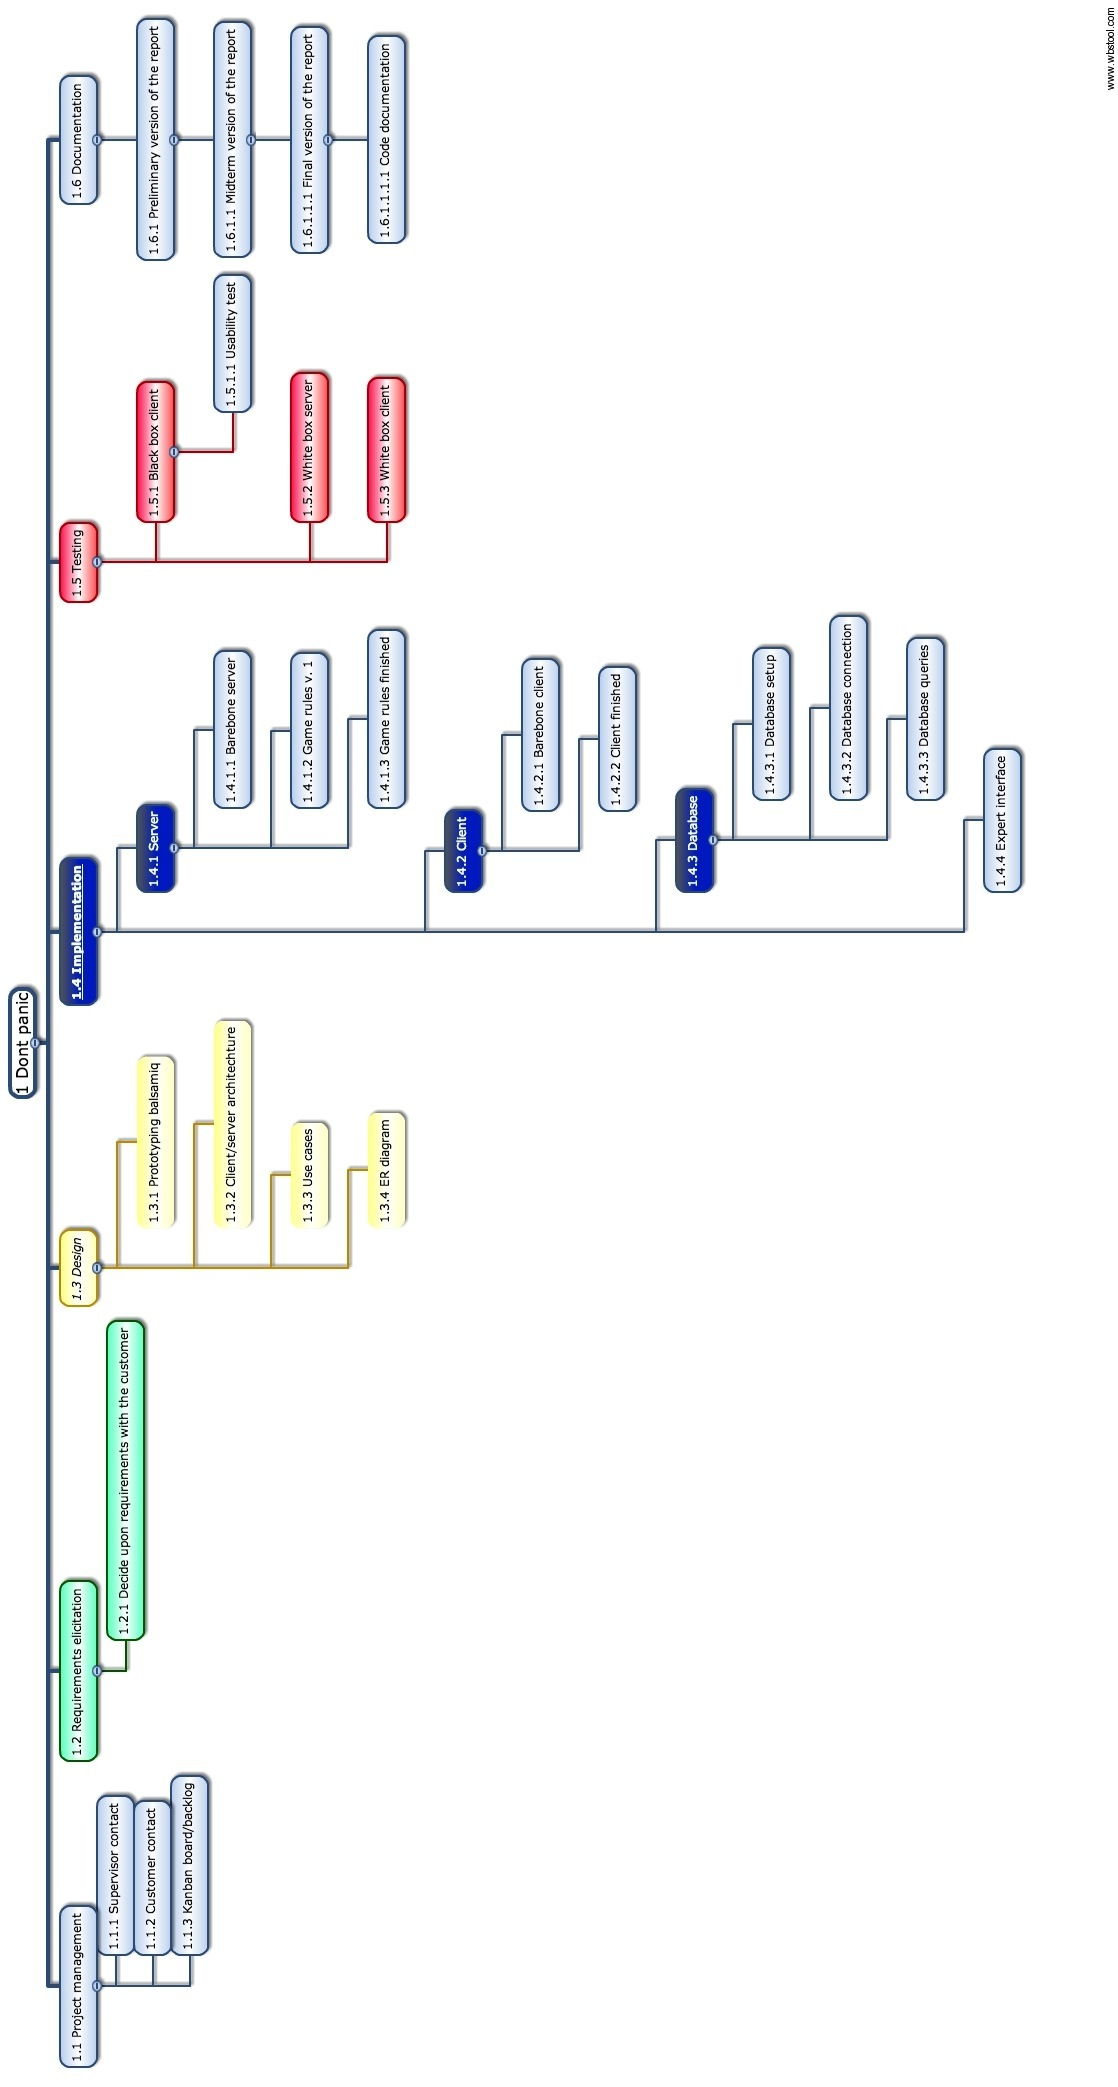
\includegraphics[width=1.0\textwidth]{img/wbs.jpeg}
  \caption{Project management, 'Work breakdown structure'} 
  \label{fig:WBS}
\end{figure}


\section{Risk list}
{\footnotesize
\begin{longtable}{| p{2.5cm} | p{1.5cm} | p{1.5cm} | p{1.5cm} | p{3cm} | p{3cm} |}\hline
	\textbf{Description} & \textbf{Likeli- hood} & \textbf{Impact (1-9)} & \textbf{Impor- tance} & \textbf{Preventive action} & \textbf{Remedialaction} \\
	\\\hline
	Data-loss (docs or code) 	& 3 & 7 & 21 
		& Continuous saving and version control. Distribute data among all group members. 
		& Try to retrieve data from computer/repository. Start from scratch, if necessary.
	\\\hline
	Network failure 			& 3 & 3 & 9  & 
		N/A & Switch to another network. Ask IDI for help, if necessary. 
	\\\hline
	Computer crash(es) & 4 & 7 & 28 & Continuous upload to repository & 
		Try to retrieve data. Worst case scenario: Retrieve most up-to-date data 
		from repository. Use computers from IDI (P15). 
	\\\hline
	Organization/ communication failure & 5 & 7 & 35  & Be watchful of correct 
		distribution of information. & Find out where communication failed and 
		restore the organization. 
	\\\hline
	Personnel absent due to sickness & 6 & 3 & 18 & Continuous upload to 
		repository. Be prepared to pitch in on others’ assignment, inform the 
		group that you are unable to meet on the day of sickness. \& Get update 
		and data from the person in question. Bring the person up-to-speed on 
		project, work done while he was away. & 
	\\\hline
	Great personal conflicts & 3 & 8 & 24 & Be prepared to withstand discussion 
		and criticism. Tell the other members of the group how you feel. Go to 
		the supervisor/ \& professor for advice if necessary. & Resolve the 
		issues with the help of a neutral part (supervisor/professor). 
	\\\hline
	Absent personnel & 7 & 3 & 21 & Point out the importance of attendance to 
		appointed hours. Inform ahead of time if leaving for vacation. See also 
		\emph{Personnel absent due to sickness}.  & Point out the importance of 
		attendance again. Notify student assistant if it becomes a problem. See 
		also \emph{Personnel absent due to sickness.}
	\\\hline
	Loss of personnel & 2 & 8 & 16 & Regular uploads of code and information 
		to repository & Notify supervisor of loss of personnel. Split work 
		assignments to personnel left in group.  
	\\\hline
	Incorrect system requirements & 3 & 8 & 24 & Be sure everyone has read and 
		understood the project requirements. Ask the customer if there any 
		uncertainties. & Resolve the incorrect requirements. Find out what went 
		wrong. Be confident that the other requirements are correct by 
		confirming with the customer.
	\\\hline
	Inexperienced with development technology & 8 & 3 & 24 & Be prepared to 
		search for information needed. Ask for help from supervisor if 
		necessary. Choose technology we are already comfortable with, if 
		possible. & Search and retrieve needed information. Get acquainted with 
		the technology needed. 
	\\\hline
	Misunderstand project & 2 & 9 & 18 & Make sure everyone has read and 
		understood the project goals, and that our goal(s) fit the customers 
		needs. Regular meetings with the customer for discussion regarding our 
		goals/customer needs. & Notify supervisor of grave errors/
		misunderstandings. Work out a rescue plan with the customer. 
	\\\hline
	Misunderstand subproblem & 2 & 8 & 16 & Make sure everyone involved has 
		read and understood the sub project problem/solution. & Correct the 
		mistakes and restart resolvement of subproblem. 
	\\\hline
	Error estimation of time needed & 5 & 5 & 25 & Be prepared for incorrect 
		time estimate, including error margins, avoid bursts. & Do bursts, 
		expand time schedules for work/work longer hours. 
	\\\hline
\caption{Risk assesment list}
\label{fig:risklist}
\end{longtable}
}


\section{Example of status report}
At the end of each week a status report will be sent to the customer and supervisor. This is an example of a status report that follows the given template: \\
\newline
Status report week 10 group 10\\
\\
\textbf{1 Introduction}\\
We now have a working prototype!\\
\\
\textbf{2 Progress summary}\\
The players can now move and de-panic zones, and turns are implemented. A timer for increased panic is implemented. The drawing functionality for objects works for the most part, and the database connection is now up and running. Css has been implemented for nice looks. Messages passing between the client and server (with json) work correctly.\\
\\
\textbf{3 Open / closed problems}\\
The database connection was a huge problem. It was detected that IDI had a firewall turned on. Much time was wasted due to error detection in the code (which was pretty much correct all the time).\\
\\
\textbf{4 Planned work for the next period}\\
Make database queries, event and information cards, roles and figure out how to implement effects (could be tricky). Produce documentation as always. Finish the requirements for the midterm report.\\
\\
\textbf{5 Updated risks analysis}\\
No updates needed.\\


\section{Communication}
During the project period it is important to continuously communicate with the customer. This way the customer is always informed on what has been done and enables giving feedback on what is desired next. In addition, the supervisor needs to be informed about the progress/work at all times. Finally, it is crucial that all team members communicate well.

\subsection{Interactions with the customer}
Regular meetings with the customer took place either weekly or bi-weekly. The meetings were scheduled through email. Prior to each meeting a presentation of the current state of the game was prepared. In addition, questions that needed answers regarding game functionality and rules were written. Simple logs of these meetings were kept to enable later reflections on the meetings. The fact that the customer is located at NTNU made it easy to set up schedules and have meetings.\\
\\
Throughout the meetings, the customer sometimes requested new tasks that went beyond the initial game functionalities. This was done because the customer was satisfied with the work so far, and wanted to provide extra challenges. These challenges were not required for this project, but if possible, they would add extra features to the game. An example of this was the possibility of using Sifteo Cubes as a game client, where the cubes would be used as zones. This was mentioned by the customer during one of the meetings. As this was not an important functionality, it was decided to focus 100\% on developing the JavaScript/HTML5 client, and perhaps test the Cubes at a later stage when the client was fully functional.



\begin{table}[H]
{\scriptsize
\begin{tabular}{|p{1.9cm}|p{1.9cm}|p{1.9cm}|p{3cm}|p{3.5cm}|p{3.5cm}|}
\hline
	\textbf{Date} & \textbf{Called by} & \textbf{Purpose} & \textbf{Preperation}
	 	& \textbf{Agenda} & \textbf{Notes} 
\\ \hline
	3/11/2013 & Customer & Update on where we are with the project
		& Implemented timer and cards (at least core functionality of cards), 
a task given to us on prior meeting 
		& Discussed how the amount of people should affect the panic level in 
the zones. Panic in a zone COULD be proportional to the amount of people, not 
important. Discussed events and how they could be solved by finishing a "quest" 
of different steps (example: if there is a fire: move people out, block zone, 
put out fire). These "quests" were not a requirement, only a suggestion. 
Discussed the use of Sifteo Cubes (an interactive game system with electronic 
gadgets) as a client, not a requirement. Important that we have a working 
game+client; other clients are "bonuses". 
		& This week we will work mostly with the report, not the game. This was explained to the customer.
\\\hline
\end{tabular}
}
\caption{Customer meeting log}
\label{fig:CustomerMeetingLog}
\end{table}

\normalsize


\subsection{Interactions with the supervisor}
The meetings with the supervisor took place bi-weekly and were scheduled through email. At these meetings the supervisor was informed about the work done since the last meeting. Problems and the group dynamic were also discussed. The supervisor provided feedback on the reports, which was much appreciated.

\subsection{Interactions within the group}
As there were meetings several times a week, much of the communication between the team members was done talking on a daily basis. In addition, meetings were planned and problems discussed through a facebook group. Facebook was chosen over e.g. email because all team members use facebook often, and long discussions through emails were regarded as messy.











